\documentclass{article}
\usepackage[utf8]{inputenc}

\title{Report.8.scatter.tex}
\author{gw.muraro}
\date{November 1st 2018}

\usepackage{natbib}
\usepackage{graphicx}
\usepackage{pgfplots}
\usepackage{minted}
\usepackage{hyperref}

\begin{document}

\maketitle
\section{Labwork 8}

\subsection{Explain how you implement the labworks}

   The goal of this labwork is to implement a scatter to pass an image from the RGB color space to HSV color space. To do so, we will pass from an array of structure (array of uchar3) to a structure of arrays (structure HSV containing 3 arrays). The implementation of the RGB to HSV color space requires a lot of conditions. These condition can be optimize by maths. We will see the two methods. 

    \begin{enumerate}     

    \item \textbf{HSV structure}
    
    The HSV structure contains three arrays of float values ($H,S,V \in [0,1]$). This structure can be declared and initiate as below : 
    
    \begin{minted}{c}
// Declaration of HSV structure
typedef struct _HSV {
    float * H ;
    float * S ;
    float * V ;
} HSV;
[...] 
// Allocation of HSV Structure 
HSV hsv ;
cudaMalloc((void **) &hsv.H, pixelCount * sizeof(float));
cudaMalloc((void **) &hsv.S, pixelCount * sizeof(float));
cudaMalloc((void **) &hsv.V, pixelCount * sizeof(float));
    \end{minted}

    \item \textbf{RGB to HSV}   
    
    This kernel function "HSV2RGB" implements the basic algorithm of HSV transformation : 
    
    \begin{minted}{c}
__global__ void RGB2HSV(
    uchar3 *input, 
    int imageWidth, 
    int imageHeight, 
    HSV hsv) {

    //getting the pixel with the second dimension
    int tidx = (threadIdx.x + blockIdx.x * blockDim.x) ; 
    int tidy = (threadIdx.y + blockIdx.y * blockDim.y) ;
    int tid = tidx + imageWidth * tidy ;
    if (tidx >= imageWidth || tidy >= imageHeight) return ;

    // floating rgb values
    float R = (float) input[tid].x /255.0 ;
    float G = (float) input[tid].y /255.0 ;
    float B = (float) input[tid].z /255.0 ;

    // Finding Min and max from our R, G or B value of our pixel
    float deltaMin = min(min(R, G), B) ;
    float deltaMax = max(max(R, G), B) ;
    float delta = deltaMax - deltaMin ;

    // Delta, also called V, can be set in our structure
    hsv.V[tid] = deltaMax ;

    // worst case scenario 
    if (deltaMax == 0 ) {
        hsv.H[tid] = 0 ;
        hsv.S[tid] = 0 ;
        return ;
    }

    // S can be set in our structure 
    hsv.S[tid] = (float) (delta/deltaMax);

    if (delta == 0) {
        hsv.H[tid] = 0 ; 
        return ;
    }


    // DEFINING H (in a silly way) ...
    if (R >= deltaMax) {
        hsv.H[tid] = fmodf((G - B)/delta, 6.0) ; 
        return ;
    }

    if (G >= deltaMax) {
        hsv.H[tid] = (2.0 + (B - R)/delta) ;
        return ;
    }

    // default case 
    if (B >= deltaMax) {
        hsv.H[tid] =(4.0 + (R - G)/delta) ;
        return  ;
    }
}
    \end{minted}
    
    This kernel can be update by suppressing the conditions. However, it requires to use maths. We will use an upgrade of the \hyperlink{http://www.daaam.info/Downloads/Pdfs/proceedings/proceedings_2011/1591_Kobalicek.pdf}{\underline{\textit{\textcolor{blue}{Lagrange polynomial}}}}.
    
    It consist on prepare one formula which will include all R, G and B, reduced to 0 and/or rightly signed. For that we use a boolean array containing the 3 conditions of utilisation of the R, G and B values. The formula manipulates signs and logical tests and seems more optimize.  
    
    \begin{minted}{c}
__device__ int sign(bool x) {
	// return 1 if > 0, 0 if 0, -1 if < 0
	return (x > 0) - (x < 0) ;
}
__global__ void RGB2HSVMaths(
    uchar3 *input, 
    int imageWidth, 
    int imageHeight, 
    float * h, 
    float *s, 
    float *v) {
    
    /* VERIFICATIONS */	[...]
    /* IMPLEMENTATION */ [...]
    /* Define S and V with the same method 
    than the classic implementation
    */
    
    /* DEFINE H */
    
    // making XYZ matrix to prepare the final formula 
    bool maxColor[3] ; 
    maxColor[0] = R != deltaMax ;
    maxColor[1] = R == deltaMax || G != deltaMax ;
    maxColor[2] = R == deltaMax || G == deltaMax ;
    if (delta == 0.0 || deltaMax == 0) {
    	h[tid] = 0 ;
    	s[tid] = 0 ;		
    	v[tid] = 0 ;
    }
    
    // Mathematical methode based on the linked paper
    
    // define H 
    float hbase = (-(4/6) && maxColor[0] ^ sign(!maxColor[2])) + 1.0 ;
    float Rm = (R && maxColor[0]) ^ sign(!maxColor[1]) ;
    float Gm = (G && maxColor[1]) ^ sign(!maxColor[2]) ;
    float Bm = (B && maxColor[2]) ^ sign( maxColor[1]) ;
    
    // Final formula 
    float H = fmod((hbase + (Rm + Gm + Bm)/(6*delta)), (float)1);
    h[tid] = H;
    s[tid] = delta/deltaMax;
    v[tid] = deltaMax;
}
    \end{minted}
    
    However, even though this method is more elegant, this particular implementation does not get the good results. 
    
    \item \textbf{HSV to RGB}
    
    The HSV to RGB implementation is pretty simple. However, the main difficulty is that we calculated radians and not degrees, so we will have to adapt our conditions. 
    
    We use M\_PI, the C language $\pi$ to pass the conditions. Every $\pi/3$, the H value has to set a different color in R, G and B. We then multiply R, G and B values by 255. 
    
    This implementation is not optimized, but we did not found any better way to do it : 
    
    \begin{minted}{c}
__global__ void HSV2RGB(
    HSV hsv, 
    int imageWidth, 
    int imageHeight, 
    uchar3 *output) {
    
	//getting the pixel with the second dimension
	int tidx = (threadIdx.x + blockIdx.x * blockDim.x) ; 
	int tidy = (threadIdx.y + blockIdx.y * blockDim.y) ;

	int tid = tidx + imageWidth * tidy ;
	
	if (tidx >= imageWidth || tidy >= imageHeight) return ;
	
	// "caching" the values
	float h = hsv.H[tid] ;
	float s = hsv.S[tid] ;
	float v = hsv.V[tid] ; // *255 easing futur multiplication 
	
	// preparation to the conditions and RGB values
	float d = h / 60;
	float hi = ((int) d % 6); 
	float f = d - hi;
	float l = v * (1.0 - s);
	float m = v * (1.0 - f * s);
	float n = v * (1.0 - ( 1.0 - f ) * s);
	
	if(h < M_PI/3) {     
	    output[tid].x = v * 255 ;
	    output[tid].y = n * 255 ;
	    output[tid].z = l * 255 ;
	    return;   
	}
   
	if(h >= M_PI/3 && h < M_PI*2/3) {     
	    output[tid].x = m * 255 ;
	    output[tid].y = v * 255 ;
	    output[tid].z = l * 255 ;
	    return;
	}
   
   
	if(h >= M_PI*2/3 && h < M_PI) {     
	    output[tid].x = l * 255 ;
	    output[tid].y = v * 255 ;
	    output[tid].z = n * 255 ;
	    return;
	}
   
   
	if(h >= M_PI && h < M_PI*4/3) {     
	    output[tid].x = l * 255 ;
	    output[tid].y = m * 255 ;
	    output[tid].z = v * 255 ;
	    return;
	}
   
   
	if(h >= M_PI*4/3 && h < M_PI*5/3) {     
	    output[tid].x = n * 255 ;
	    output[tid].y = l * 255 ;
	    output[tid].z = v * 255 ;
	    return;
	}
       
	if(h >= M_PI*5/3) {
	    output[tid].x = v * 255 ;
	    output[tid].y = l * 255 ;
	    output[tid].z = m * 255 ;
	    return;
	}
}
    \end{minted}
    
    \end{enumerate}

\subsection{Results}

    By using a bash script and adapting our code to receive a 3$^{rd}$ argument precising the block Number in 2D, we got these results : 

    \begin{verbatim}
==== 2D Block Number : 2
USTH ICT Master 2018, Advanced Programming for HPC.
Warming up...
Starting labwork 8
labwork 8 with scatter ellapsed 48.1ms

==== 2D Block Number : 4
USTH ICT Master 2018, Advanced Programming for HPC.
Warming up...
Starting labwork 8
labwork 8 with scatter ellapsed 34.9ms

==== 2D Block Number : 16
USTH ICT Master 2018, Advanced Programming for HPC.
Warming up...
Starting labwork 8
labwork 8 with scatter ellapsed 32.2ms

==== 2D Block Number : 32
USTH ICT Master 2018, Advanced Programming for HPC.
Warming up...
Starting labwork 8
labwork 8 with scatter ellapsed 32.3ms

    \end{verbatim}

\subsection{Plot a graph}
    
   %%plot
    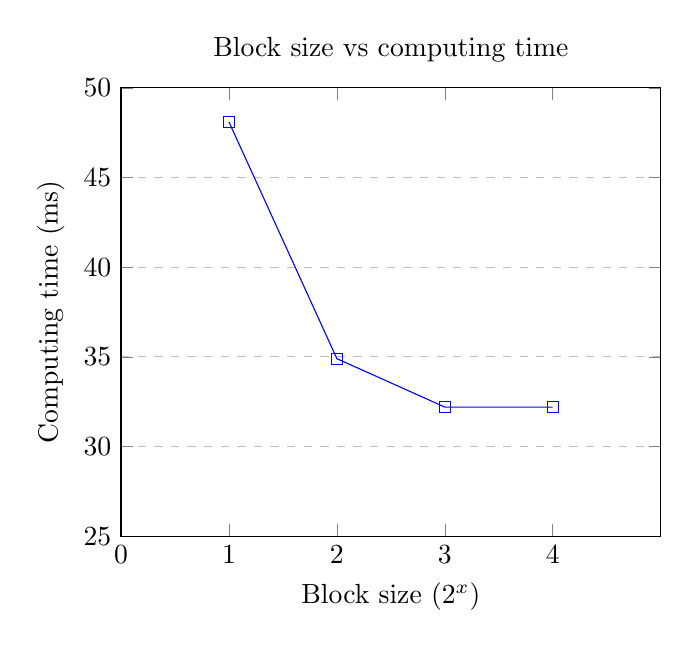
\begin{tikzpicture}
        \centering
        %%define axes
        \begin{axis}[
            title={Block size vs computing time},
            xlabel={Block size ($2^x$)},
            ylabel={Computing time (ms)},
            xmin=0, xmax=5,
            ymin=25, ymax=50,
            xtick={0,1, 2, 3, 4},
            ytick={25, 30, 35, 40, 45, 50},
            legend pos=north east,
            ymajorgrids=true,
            grid style=dashed,
        ]
        %% data filing
        \addplot[color=blue, mark=square]
            coordinates { %% Remind : axis X = 2^x
                (1,48.1)(2,34.9)(3,32.2)(4,32.2)
            };
        \end{axis}
    \end{tikzpicture}
    \newline


\end{document}

